\subsection{Ecuaciones en diferencias}

\begin{frame}
\frametitle{Ecuaciones en diferencias(E.D)}
\begin{block}{Definición 1:}
Una ecuación en diferencias es una expresión de la forma: \[ G\left(n,f(n),f\left(n+1\right),\ldots,f\left(n+k\right)\right)=0,\quad\forall n\in\mathds{Z}. \]
\emph{Obs:} $f$ está definida en $\mathds{Z}$.
\end{block}

\begin{block}{Definición 2:}
Se le llama orden de una E.D a la diferencia entre el operador diferencia mayor y menor que aparezcan en la ecuación; es decir, $n+k-n=k$.
\end{block}

\begin{block}{Ejemplo}
$f\left(n+3\right)-f\left(n+1\right)-5f(n)=n$ es una E.D de orden $3$.

$f\left(n+3\right)-f\left(n+1\right)=n^{2}-3$ es una E.D de orden $2$.
\end{block}
\end{frame}

\begin{frame}
\begin{block}{Definición 3:}
Se le llama \emph{solución} de una E.D a toda sucesión $\{f\left(0\right),f\left(1\right),\ldots,f(n),\ldots\}$ que la satisfaga, ahora se le llama \emph{solución general} de una E.D al conjunto de todas las soluciones que tendrán tanto parámetros como orden tenga la ecuación. La determinación de estos parámetros, a partir de unas condiciones iniciales, nos proporcionará las distintas soluciones particulares.
\end{block}

\begin{block}{Ejemplo 3.1:}
$f\left(n+1\right)-f\left(n\right)=3$ es una E.D de orden uno cuya solución general es $f\left(n\right)=3n+c$. Si consideramos unas condiciones iniciales, por ejemplo, $f(0)=2$, entonces $f(0)=3\times0+c=c$, por tanto $c=2$ y la solución particular es $f_{p}(n)=3n+2$. Es decir, la solución es la sucesión $f_{p}(n)=\left\{2,5,8,11,\ldots\right\}$.
\end{block}
\end{frame}

\begin{frame}
\begin{block}{Ecuaciones en diferencias lineales(E.D.L)}
Llamamos ecuación en diferencias lineal de orden $k$ a toda expresión de la forma:
\[ f\left(n+k\right)+a_{1}(n)f\left(n+k-1\right)+\cdots+a_{k-1}(n)f\left(n+1\right)+a_{k}(n)f\left(n\right)=b\left(n\right) \]
\emph{Obsv:} $a_{k}(n)\neq0$.
\end{block}

\begin{block}{Clasificación:}
Las E.D.L se pueden clasificar en:

\begin{itemize}
	\item Homogéneas si $b(n)=0$.
	\item Completas si $b(n)\neq0$.
	\item De coeficientes constantes si $a_{i}(n)=a_{i}$, $\forall i$.
	\item De coeficientes no constantes si $a_{i}(n)\neq a_{i}$ para algún $i$.
\end{itemize}
\end{block}
\end{frame}

\begin{frame}
\begin{block}{Teorema 1:{\bf (Teorema de la existencia y la unicidad)}}
Dada la ecuación: \[ f\left(n+k\right)+a_{1}(n)f\left(n+k-1\right)+\cdots+a_{n-1}(n)f\left(n+1\right)+a_{n}(n)f\left(n\right)=0, \] y dados $n$ números reales $k_{0}$, $k_{1}$, \ldots, $k_{n-1}$ existe una única solución que verifica \[ f\left(0\right)=k_{0},f\left(1\right)=k_{1},\ldots,f\left(n-1\right)=k_{n-1}. \]
\end{block}

\begin{block}{Teorema 2:}
Toda combinación lineal de soluciones de una ecuación en diferencias lineal homogénea de orden $n$ es también una solución.
\end{block}

\begin{block}{Corolario 1:}
Las soluciones de una ecuación en diferencia lineal de orden $n$ forman un espacio vectorial.
\end{block}

\begin{block}{Teorema 3:}
La dimensión del espacio de soluciones de una ecuación en diferencias lineal de orden $n$ es $n$.
\end{block}
\end{frame}

%http://personal.us.es/pnadal/Informacion/leccion5ecdiferencias.pdf
\begin{frame}
\begin{block}{Ecuaciones en diferencias de primer orden}
\end{block}

\begin{block}{Ecuaciones en diferencias de segundo orden}
\end{block}
\end{frame}

\subsubsection{Número de Catalan}

\begin{frame}{Número de Catalan}
\begin{block}{Triangulación}
	\begin{figure}
	\centering
	
\includegraphics[scale=0.15]{ca1}
	\end{figure}
\end{block}

\begin{block}{Caminos monótonos}
	\begin{figure}
	\centering
	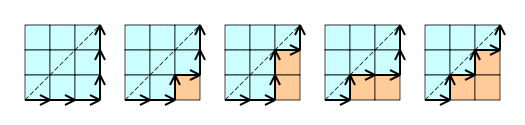
\includegraphics[scale=0.25]{ca2}
	\end{figure}
\end{block}
\end{frame}